\thispagestyle{empty}
\section*{Preambule}

\begin{figure}[h]
  \centering

  % \caption{An old painting of Isaac Newton writing the theory of gravity in the language of probability and questioning the role of models in the world. Made by $\text{DALL}\cdot\text{E }2$.}
  \includegraphics[width=.95\textwidth]{/Users/awehenkel/Documents/Ecole/2021-2022/phd-thesis/tex/figures/chapter02/430122767_A_highly_detailed_painting_of_a_humanoid_robot_in_iron_that_has_the_same_moustache_as_Albert_Einstein_with_the_universe_around_him_orbiting_with_maths_symbols_.png}
  \label{}
\end{figure}

\vfill

{
\textit{\justify
   The basic laws of the universe are simple, but because our senses are limited, we can't grasp them. There is a pattern in creation.}

  \par\bigskip
  \raggedleft\MakeUppercase{Albert Einstein}\\
  \par%
}

\chapter{Deep probabilistic models}\label{ch:02}

\begin{chapter_outline}

This chapter comprehensively reviews various strategies to parameterise probabilistic models with neural networks. We present the main algorithms used in practice, and we discuss the pros and cons of each class of models.
Clearly, the distinction between two models is sometimes artificial. It is why, we try to draw relevant connections between these strategies when possible.
Our aim is to convince the reader of the effectiveness and flexibility of deep probabilistic models. Finally, we provide the primary motivations for the contributions presented in this thesis.
\end{chapter_outline}

\section{Introduction}
Restricted Botzmann Models are arguably one of the first generative models built upon neural networks. This chapter discusses other successful approaches for parameterising probabilistic models with neural networks. While graphical models describe probabilistic models with graphs and are appealing for understanding and prescribing modelling assumptions, they do not rigorously describe efficient parameterisations of the conditional probability distributions in the continuous setting. Deep probabilistic models encompass methods for parameterising these probability distributions with neural networks. Some of these models are particularly well suited for sample generation and are called \textit{deep generative models}. We will highlight the correspondence of some of these models within the probabilistic graphical models when possible.

\section{Why neural networks?}
We abstract neural networks as parametric functions that map an input space $\mathcal{X}$ to an output space $\mathcal{Y}$ and are differentiable functions $f_{\bm{\theta}}: \mathcal{X} \rightarrow \mathcal{Y}$ of their parameters $\bm{\theta}$. Although neural networks are universal function approximators, the parameterisation of a probability distribution is challenging and requires the right architectural choices. We often present neural networks as deterministic models; however, many strategies exist to parameterise probability distributions, as we will see in the next sections.

For example, Normalizing flows are neural networks that directly parameterise the probability distribution but require strong architectural constraints, as we will see later. This is particularly inconvenient when working with structured data (e.g. images, sound, graphs, etc.) because specialised architectures (e.g. convolutions) do not directly satisfy the architectural constraints. Another possibility is to use a neural network to parameterise a known distribution such as a Gaussian. For example, we can model $P(Y|X)$ as a multivariate Gaussian $\mathcal{N}(\bm{\mu}, \Sigma)$ where a free-form neural network computes the mean vector and covariance matrix as a parametric function of the input $X$. This strategy makes a strong assumption in the form of $P(Y\mid X)$, which may be inaccurate, e.g. if $X$ is a piece of text describing the image $Y$. An alternative is to see the neural networks as a generator of samples similar to the training set, mapping a noise vector to realisations. These deep generative models define the probability distribution implicitly and allow us to use complex architectures well suited to the modelling task but require specialised training algorithms, as we will see in details soon.

Neural networks are better suited to parameterise distributions than other machine learning models. In particular, their differentiability and training procedure based on stochastic gradient descent allows us to optimise objectives corresponding to the MLE or MAP directly. In parallel, considerable efforts have been made over the last year to create architectures with inductive biases adapted to different data types. The availability of large pre-trained models is another advantage of working with neural networks. For example, Dall-e 2~\citep{ramesh2022hierarchical} combines a large pre-trained language model with annotated images to train a text-to-image probabilistic model.

In the following we will mostly ignore the conditioning variable $X$ as challenges in modelling distributions with neural networks is usually orthogonal to handling conditioning variables. Instead we focus on the modelling of the joint distributions of a $d$-dimensional random vector $Y = \left[Y_1, \dots, Y_d  \right]$ that takes value in $\mathcal{Y} = \mathcal{Y}_1 \times \dots \times \mathcal{Y}_d$. For simplicity, we consider that $\mathcal{Y}_1 = \dots = \mathcal{Y}_d$ and the domains are either discrete classes (e.g. a pixel value in $\{0, \dots, 255\}^3$) or real numbers $\mathbb{R}$.
\section{Autoregressive models} \label{subsec:AM}
\begin{figure}

\centering
\tikzset{every picture/.style={line width=0.75pt}} %set default line width to 0.75pt
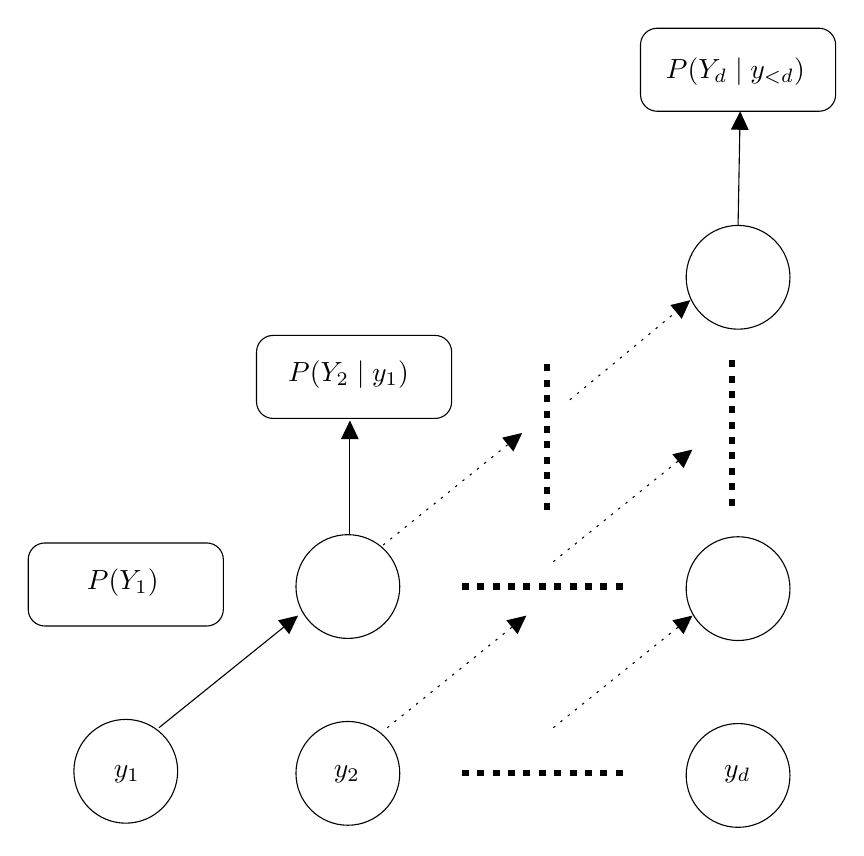
\begin{tikzpicture}[x=0.75pt,y=0.75pt,yscale=-1,xscale=1]
%uncomment if require: \path (0,453); %set diagram left start at 0, and has height of 453

%Shape: Circle [id:dp6693448840170049]
\draw   (24,394) .. controls (24,380.19) and (35.19,369) .. (49,369) .. controls (62.81,369) and (74,380.19) .. (74,394) .. controls (74,407.81) and (62.81,419) .. (49,419) .. controls (35.19,419) and (24,407.81) .. (24,394) -- cycle ;
%Shape: Circle [id:dp9581265567241148]
\draw   (131,395) .. controls (131,381.19) and (142.19,370) .. (156,370) .. controls (169.81,370) and (181,381.19) .. (181,395) .. controls (181,408.81) and (169.81,420) .. (156,420) .. controls (142.19,420) and (131,408.81) .. (131,395) -- cycle ;
%Straight Lines [id:da9687497897729951]
\draw [line width=2.25]  [dash pattern={on 2.53pt off 3.02pt}]  (211,395) -- (290,395) ;
%Straight Lines [id:da4419677445778909]
% \draw [line width=2.25]  [dash pattern={on 2.53pt off 3.02pt}]  (211,55) -- (290,55) ;
%Rounded Rect [id:dp7960962003110323]
\draw  [shift={(0,250)}] (2,42) .. controls (2,37.58) and (5.58,34) .. (10,34) -- (88,34) .. controls (92.42,34) and (96,37.58) .. (96,42) -- (96,66) .. controls (96,70.42) and (92.42,74) .. (88,74) -- (10,74) .. controls (5.58,74) and (2,70.42) .. (2,66) -- cycle ;
%Rounded Rect [id:dp544597590880084]
\draw  [shift={(0,150)}] (112,42) .. controls (112,37.58) and (115.58,34) .. (120,34) -- (198,34) .. controls (202.42,34) and (206,37.58) .. (206,42) -- (206,66) .. controls (206,70.42) and (202.42,74) .. (198,74) -- (120,74) .. controls (115.58,74) and (112,70.42) .. (112,66) -- cycle ;
%Rounded Rect [id:dp9375363954367466]
\draw   (297,44) .. controls (297,39.58) and (300.58,36) .. (305,36) -- (383,36) .. controls (387.42,36) and (391,39.58) .. (391,44) -- (391,68) .. controls (391,72.42) and (387.42,76) .. (383,76) -- (305,76) .. controls (300.58,76) and (297,72.42) .. (297,68) -- cycle ;
%Shape: Circle [id:dp9573206034482791]
\draw   (131,305) .. controls (131,291.19) and (142.19,280) .. (156,280) .. controls (169.81,280) and (181,291.19) .. (181,305) .. controls (181,318.81) and (169.81,330) .. (156,330) .. controls (142.19,330) and (131,318.81) .. (131,305) -- cycle ;
%Straight Lines [id:da8567301316866047]
\draw [line width=2.25]  [dash pattern={on 2.53pt off 3.02pt}]  (211,305) -- (290,305) ;
%Straight Lines [id:da48825283468137703]
\draw [line width=2.25]  [dash pattern={on 2.53pt off 3.02pt}]  (252,198) -- (252,270) ;
%Straight Lines [id:da4548829701939858]
\draw    (65,373) -- (129.66,320.88) ;
\draw [shift={(132,319)}, rotate = 141.13] [fill={rgb, 255:red, 0; green, 0; blue, 0 }  ][line width=0.08]  [draw opacity=0] (8.93,-4.29) -- (0,0) -- (8.93,4.29) -- cycle    ;
%Straight Lines [id:da49081615287245617]
\draw  [dash pattern={on 0.84pt off 2.51pt}]  (175,373) -- (239.66,320.88) ;
\draw [shift={(242,319)}, rotate = 141.13] [fill={rgb, 255:red, 0; green, 0; blue, 0 }  ][line width=0.08]  [draw opacity=0] (8.93,-4.29) -- (0,0) -- (8.93,4.29) -- cycle    ;
%Straight Lines [id:da9305605534968759]
\draw  [dash pattern={on 0.84pt off 2.51pt}]  (173,285) -- (237.66,232.88) ;
\draw [shift={(240,231)}, rotate = 141.13] [fill={rgb, 255:red, 0; green, 0; blue, 0 }  ][line width=0.08]  [draw opacity=0] (8.93,-4.29) -- (0,0) -- (8.93,4.29) -- cycle    ;
%Shape: Circle [id:dp9092410420976149]
\draw   (319,396) .. controls (319,382.19) and (330.19,371) .. (344,371) .. controls (357.81,371) and (369,382.19) .. (369,396) .. controls (369,409.81) and (357.81,421) .. (344,421) .. controls (330.19,421) and (319,409.81) .. (319,396) -- cycle ;
%Shape: Circle [id:dp20606971755388614]
\draw   (319,306) .. controls (319,292.19) and (330.19,281) .. (344,281) .. controls (357.81,281) and (369,292.19) .. (369,306) .. controls (369,319.81) and (357.81,331) .. (344,331) .. controls (330.19,331) and (319,319.81) .. (319,306) -- cycle ;
%Straight Lines [id:da8117853843319638]
\draw [line width=2.25]  [dash pattern={on 2.53pt off 3.02pt}]  (341,196) -- (341,268) ;
%Straight Lines [id:da9043715008310824]
\draw    (157,280) -- (157,228) ;
\draw [shift={(157,225)}, rotate = 90.28] [fill={rgb, 255:red, 0; green, 0; blue, 0 }  ][line width=0.08]  [draw opacity=0] (8.93,-4.29) -- (0,0) -- (8.93,4.29) -- cycle    ;
%Straight Lines [id:da6288348052624073]
\draw  [dash pattern={on 0.84pt off 2.51pt}]  (263,215) -- (318.69,168.91) ;
\draw [shift={(321,167)}, rotate = 140.39] [fill={rgb, 255:red, 0; green, 0; blue, 0 }  ][line width=0.08]  [draw opacity=0] (8.93,-4.29) -- (0,0) -- (8.93,4.29) -- cycle    ;
%Shape: Circle [id:dp08259847117385988]
\draw   (319,156) .. controls (319,142.19) and (330.19,131) .. (344,131) .. controls (357.81,131) and (369,142.19) .. (369,156) .. controls (369,169.81) and (357.81,181) .. (344,181) .. controls (330.19,181) and (319,169.81) .. (319,156) -- cycle ;
%Straight Lines [id:da7091929499334224]
\draw    (344,131) -- (344.95,79) ;
\draw [shift={(345,76)}, rotate = 91.04] [fill={rgb, 255:red, 0; green, 0; blue, 0 }  ][line width=0.08]  [draw opacity=0] (8.93,-4.29) -- (0,0) -- (8.93,4.29) -- cycle    ;
%Straight Lines [id:da5760019375125367]
\draw  [dash pattern={on 0.84pt off 2.51pt}]  (255,373) -- (319.66,320.88) ;
\draw [shift={(322,319)}, rotate = 141.13] [fill={rgb, 255:red, 0; green, 0; blue, 0 }  ][line width=0.08]  [draw opacity=0] (8.93,-4.29) -- (0,0) -- (8.93,4.29) -- cycle    ;
%Straight Lines [id:da731846091518092]
\draw  [dash pattern={on 0.84pt off 2.51pt}]  (255,293) -- (319.66,240.88) ;
\draw [shift={(322,239)}, rotate = 141.13] [fill={rgb, 255:red, 0; green, 0; blue, 0 }  ][line width=0.08]  [draw opacity=0] (8.93,-4.29) -- (0,0) -- (8.93,4.29) -- cycle    ;

% Text Node
\draw (29,295) node [anchor=north west][inner sep=0.75pt][align=left] {$\displaystyle P( Y_{1})$};
% Text Node
\draw (126,195) node [anchor=north west][inner sep=0.75pt][align=left] {$\displaystyle P( Y_{2} \mid y_{1})$};
% Text Node
\draw (42,390) node [anchor=north west][inner sep=0.75pt]   [align=left] {$\displaystyle y_{1}$};
% Text Node
\draw (148,390) node [anchor=north west][inner sep=0.75pt]   [align=left] {$\displaystyle y_{2}$};
% Text Node
\draw (308,49) node [anchor=north west][inner sep=0.75pt] [align=left] {$\displaystyle P( Y_{d} \mid \bm{y}_{< d})$};
% Text Node
\draw (336,390) node [anchor=north west][inner sep=0.75pt]   [align=left] {$\displaystyle y_{d}$};


\end{tikzpicture}
\caption{The forward computation of an autoregressive model. Each 1D distribution is conditioned autoregressively on the input vector.}
\end{figure}
Autoregressive models reduce the modelling of $d$-dimensional distributions into $d$ distributions via the product rule ($P(A, B) = P(A) P(B\mid A)$). The autoregressive structure is there to account for the piling-up conditioning factors. These models can represent all kinds of dependencies between the components of the random vector modelled.
Formally, autoregressive models decompose the joint distribution as
\begin{align}
  P(Y) = P(Y_1) \Pi^d_{i=2} P(Y_i|Y_{<i}), \quad \text{where} \quad Y_{<i} \triangleq \left[ Y_1, \dots, Y_{i-1}\right].
\end{align}
When the domain is discrete, we can parameterise each $1$D factor with a classifier. If the domain is continuous, the common practice is to parameterise a $1$D Gaussian distribution with a neural network that predicts the mean and log-variance given the conditioning vector. Mixture density networks~\citep[][MDNs]{bishop1994mixture} are an effective alternative that easily accounts for multimodality. MDNs parameterise a mixture of $m$ $1D$ distributions (e.g., Gaussian distributions) with a neural network that assigns a normalised weight to each mixture component, in addition to their parameters (e.g. the mean and log-variance).
An autoregressive model naturally leads to the parameterization of $d$ functions with different input dimensionalities which might be very inefficient if $d$ is large (e.g. $2^{16}$ for $256\times256$ images).

Sharing parameterisation between factors is an important aspect of autoregressive models. One strategy is to use recurrent neural networks where the hidden vector carries and updates the information of the successive conditioning variables\citep{van2016pixel}. However, this strategy is slow because it processes the input vector sequentially. Moreover, the inductive bias of recurrent neural networks is not ideal for signals with long-range or spatial dependencies such as audio or images. A better solution is to use causal convolutional neural networks (CNNs), which process the complete vector simultaneously and enforce the autoregressive structure in the outputs. Causal CNNs have achieved great success in modelling audio \citep{van_den_oord_wavenet_2016, van_den_oord_parallel_2018}. The PixelCNN autoregressive model generalises this architecture to 2D signals and has shown great modelling capabilities\citep{oord_conditional_2016}.

We can train autoregressive models efficiently by maximising their likelihood given data. Evaluating the likelihood only requires passing the data once in the network and computing the product of the $d$ conditional distribution evaluated at the input vectors. Unfortunately, sampling is a sequential process as each variable is sampled according to the preceding. This is particularly slow for images or long time series and is one of the main drawbacks of autoregressive models. The lack of independence assumptions and poor inductive bias are additional limitations of these models. This is especially true with images for which the enforced causality between successive pixels and sampling algorithm is ineffective. We rarely use autoregressive models alone but in combination with other models, such as variational auto-encoders.

% \textcolor{red}{Add an image that describes the sampling procedure of autoregressive nets.}
\section{Energy based models} \textcolor{red}{upgrade with info in Kingma's paper and explicitly say that we are strongly inspired by them.}
\begin{figure*}
  \centering
  \begin{subfigure}{.48\textwidth}
    \centering
    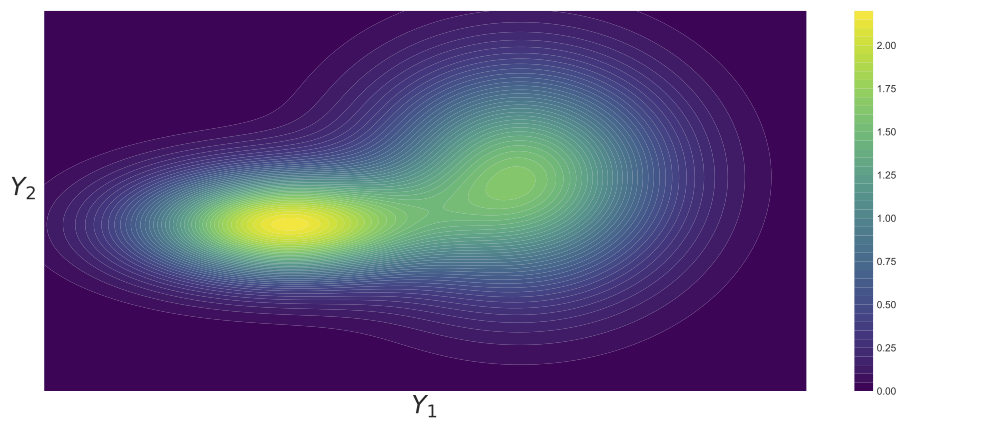
\includegraphics[width=.95\textwidth]{figures/chapter02/energy-landscape.pdf}
    \caption{}
    \label{fig:Energy}
  \end{subfigure}
  \begin{subfigure}{.48\textwidth}
    \centering
    \includegraphics[width=.95\textwidth]{figures/chapter02/pdf-landscape.pdf}
    \caption{}
    \label{fig:pdf}
  \end{subfigure}
  \caption{The energy landscape of a 2D bi-modal distribution (\textbf{a}) and the corresponding probability density function (\textbf{b}).}
\end{figure*}
We have already encountered the term \textit{energy} when discussing the parameterisation of Markov networks. There, and in the context of energy-based models (EBM), the energy relates to the definition of a Gibbs distribution, taking the form
\begin{align}
  P_{\bm{\theta}}(Y=\bm{y}) = \frac{1}{Z(\bm{\theta})} e^{-E_{\bm{\theta}}(\bm{y})},
\end{align}
where $E_{\bm{\theta}}(\cdot): \mathcal{Y}\rightarrow \mathbb{R}$ is the energy function and $Z(\bm{\theta})$ is called the partition function. \Cref{fig:Energy} shows the energy function of a 2D distribution with two modes, the integral over the support is not equal to $1$, but the energy is proportional to the logarithm of the probability density function.

The interest of EBMs is to parameterise probability distributions with free-form real functions. For instance, any neural network can potentially parameterise an EBM. This property is particularly appealing as it allows combining the flexibility and efficient inductive bias of neural networks, which was fundamental reasons for the greatest successes of deep learning. Unfortunately, this flexible parameterisation prevents direct access to the likelihood function, which requires the intractable computation of the partition function. This prevents the direct application of the classical MLE learning strategy. We now review the main approaches for learning EBMs for continuous variables.

\subsection{Markov chain Monte Carlo}
In order to find the best set of parameters $\bm{\theta}$, we need to evaluate $P_{\bm{\theta}}$ and potentially its derivative, not only the energy function.
A natural strategy would be to compute the integral $\int_{y\in \mathcal{Y}}e^{-E_{\bm{\theta}}(\bm{y})} \text{d}y$. However, as soon as the energy function is non-trivial, this integral becomes intractable. Thus, we need to find a better strategy. We see below how sampling from the EBM can save us the pain to explicitly compute $Z(\bm{\theta})$.

Let us formalise the learning problem for a given dataset $\mathcal{D} := \{\bm{y}_i\}_{i=1}^N$ of $N$ iid samples. A reasonable strategy is to find the MLE,
\begin{align}
  \theta^\star &= \argmax_\theta P_{\bm{\theta}}(\mathcal{D})\\
  &= \argmax_\theta \log P_{\bm{\theta}}(\mathcal{D})\\
  &= \argmax_\theta \frac{1}{N} \sum^N_{i=1} \log P_{\bm{\theta}}(Y=\bm{y}_i).
\end{align}
In practice we cannot solve this last equation directly and we would like to use standard optimization techniques such as (stochastic) gradient ascent. In this case, learning the EBMs eventually reduces to being able to evaluate $\nabla_{\bm{\theta}} \log P_{\bm{\theta}}(Y=\bm{y}_i)$ for any $\bm{y}_i \in \mathcal{D}$. Unfortunately, this gradient explicitly depends on the parition function,
\begin{align}
  \nabla_{\bm{\theta}} \log P_{\bm{\theta}}(\bm{y}) = \nabla_{\bm{\theta}} \log Z(\bm{\theta}) -\nabla_{\bm{\theta}} E_{\bm{\theta}}(\bm{y}).
\end{align}

However, we can rewrite the problematic term as an expectation over samples from the EBMs:
\begin{align}
\nabla_{\bm{\theta}} \log Z(\bm{\theta}) &= \nabla_{\bm{\theta}} \log \int_{\bm{y}\in \mathcal{Y}}e^{-E_{\bm{\theta}}(\bm{y})} \text{d}\bm{y}\\
&= \left( \int_{\bm{y}\in \mathcal{Y}}e^{-E_{\bm{\theta}}(\bm{y})} \text{d}\bm{y} \right)^{-1} \int_{\bm{y}\in \mathcal{Y}}
\nabla_{\bm{\theta}}\left( e^{-E_{\bm{\theta}}(\bm{y})}  \right) \text{d}\bm{y}\\
&= \int_{\bm{y}\in \mathcal{Y}} \underbrace{\left( \int_{\bm{y}\in \mathcal{Y}}e^{-E_{\bm{\theta}}(\bm{y})} \text{d}\bm{y} \right)^{-1}
e^{-E_{\bm{\theta}}(\bm{y})}}_{=P_{\bm{\theta}}(\bm{y})} \nabla_{\bm{\theta}}\left(-E_{\bm{\theta}}(\bm{y})\right) \text{d}\bm{y}\\
&= -\mathbb{E}_{P_{\bm{\theta}}(\bm{y})}\left[ \nabla_{\bm{\theta}}E_{\bm{\theta}}(\bm{y}) \right].
\end{align}
Then, we can use MCMC to sample from the EBM and estimate the gradient of the log-likelihood function. There exist MCMC algorithms, such as Langevin MCMC~\citep{parisi1981correlation, grenander1994representations} or Hamiltonian Monte Carlo~\citep{duane1987hybrid, neal2011mcmc}, that are specifically designed to exploit the fact that the score function $\nabla_{\bm{y}} \log P_{\bm{\theta}}(\bm{y}) = -\nabla_{\bm{y}} E_{\bm{\theta}}(\bm{y})$ is directtly accessible. These algorithms are usually more efficient than Metropolis-Hastings MCMC~\citep{hastings1970monte}.

Clearly, running MCMC until convergence is expensive. Hence, the requirement to do it at each gradient step leads to inneficient learning algorithms. It is why, many improvements to the naive learning strategy, which starts each MCMC run from scracth, has been proposed. For example, contrastive divergence~\citep{hinton2002training} starts each chain from a data point rather than a random initial state. A similar strategies named persistant contrastive divergence~\citep{tieleman2008training} use persistant states between successive gradient estimations and update steps.
%
% A simple strategy is to approximate the normalising factor (and its first order derivative) with Monte Carlo estimation to perform MLE by gradient descent. However, this requires samples from the energy-based model, which is not immediate either. A solution is to resort to sampling strategies that work with unnormalised distributions, such as MCMC techniques. In practice, this strategy may work but requires tuning many hyperparameters.

\subsection{Contrastive learning}
In highly-dimensional spaces, or even for low-dimensional and multimodal distributions, sampling is often inneficient. Although strategies to improve the efficiency of MCMC-based training exists, it often leads to biased gradient estimates. This observation has motivated the development of alternative learning strategies. For instance, \citet{gutmann2012noise} proposed noise contrastive learning which estimate the partition and energy functions jointly. To do so, \citet{gutmann2012noise} notice that if the energy function models correctly the training distribution, it enables discriminating between noise and samples from the distribution.

Let us consider a balanced binary classification problem where samples from class $C=0$ follow a known noise distribution $P_n$, and class $C=1$ is the training set which follows the unknown distribution $P(Y)$. As long as the supports of the noise and the training distributions match, we can learn a Bayes optimal classifier as a function of the ratio between the two densities. This classifier attributes the posterior probabiliy to $C$ given a sample $\mathbf{y}$ as
\begin{align}
  P(C=0 \mid \mathbf{y}) = \frac{P_n(\mathbf{y})}{P_n(\mathbf{y}) + P(\mathbf{y})}. \label{eq:CL}
\end{align}
We can replace $P(\mathbf{y})$ by the EBM $P_{\bm{\theta}}(\bm{y})$ and solve the corresponding classification problem as a function of the EBM's parameters $\bm{\theta}$ and of the normalizing constant $\alpha \triangleq Z(\bm{\theta})$.

Then learning corresponds to minimising a cross-entropy loss of a classifier expressed as a function of the EBM. In practice, this strategy is sensitive to the distribution of the noise. Indeed, the cross-entropy loss is more sensitive to errors on $P_{\bm{\theta}}(\bm{y})$ in regions where the data and the noise distributions overlap. Intuitively, in low-density region of the noise, the classification is simple because $P_n(\mathbf{y})$ is very small. Hence the sensitivity of \Cref{eq:CL} to $P_{\bm{\theta}}(\bm{y})$ is small. In contrast, in high-density regions of both the noise and data distributions, the discriminator is very sensitive to errors in $P_{\bm{\theta}}(\bm{y})$.

The sensitivity of contrastive learning makes it challenging for high-dimensional data which often lives in manifold which corresponds to low-density regions of tractable noise distributions. It is why many methods to automatically tune the noise distribution have been proposed, e.g., \citep{bose2018adversarial, ceylan2018conditional, gao2020flow}.
% For instance, let us consider a point $\mathbf{y}_1$ that lives in a low-density region of the noise, e.g. $P_n(\mathbf{y}_1) = 10^-5$. If we had access the other samples comes from a higher density region $P(\mathbf{y}_1) = 0.5$. Let us suppose an EBM that attributes an equal probability $P_{\bm{\theta}}(\bm{y}_1) = P_{\bm{\theta}}(\bm{y}_2) = 0.1$

% In particular, the cross-entropy loss is not very sensitive to enforce different if samples are too simple to discriminate, e.g. if data samples corresponds to low-density regions of the noise distribution, then   .
% We can roughly interpret generative adversarial networks (GANs) as some contrastive learning of an EBM where the noise distribution is the generator and evolves along with training. The discriminator implicitly defines the energy function. Similarly, \citet{grathwohl2019your} noticed that any classifier could be seen as an EBM. It is interesting to note that contrastive learning could be particularly well suited for transferring an explicit generative model to a new dataset with similar support.

\subsection{Score matching}
Score matching \citep{hyvarinen2005estimation} fixes the innacuracy of contrastive learning in low density regions of the noise distribution. This training strategy notices that the score function, the gradient of the log-likelihood with respect to the data, is independent from the partition function. Thus learning a good energy function can be achieved by minimizing the distance between the model score function $-\nabla_Y E_{\bm{\theta}}(Y=\cdot): \mathbb{R}^d \rightarrow \mathbb{R}^d$, and the data score function $\bm{s}(\cdot)\triangleq \nabla_Y \log P(Y=\cdot): \mathbb{R}^d \rightarrow \mathbb{R}^d$. Formally this leads to the following optimization problem
\begin{align}
  \bm{\theta}^{\star} = \argmin_{\bm{\theta}} \int_{\bm{y} \in \mathbb{R}^d} P(Y=\bm{y}) \lVert \bm{s}(\bm{y}) + \nabla_Y E_{\bm{\theta}}(\bm{y})\rVert^2 \text{d}\bm{y}. \label{eq:score_matching}
\end{align}
This formulation is still difficult to optimise as it would require accessing the data's score function, which is what we are implicitly trying to estimate by learning the energy function. However, under weak regularity conditions, we can express the objective function in \Cref{eq:score_matching} as
\begin{align}
  J(\bm{\theta}) = \int_{\bm{y} \in \mathbb{R}^d} P(Y=\bm{y}) \sum_{i=1}^d \left[ \frac{-\partial \nabla_Y E_{\bm{\theta}}[i]}{\partial y_i } + \frac{1}{2} (\nabla_Y E_{\bm{\theta}[i]})^2 \right] \text{d}\bm{y} + C,
\end{align}
where $\nabla_Y E_{\bm{\theta}}[i] = \frac{\partial E_{\bm{\theta}}}{\partial y_i}$ is the partial derivative of the energy function with respect to the $\text{i}^{\text{th}}$ component of the input vector $\bm y$. The constant $C$ is independent from the parameters $\bm \theta$. In the case where we use neural networks to parameterise the energy function, the objective function directly translates into a loss function. We note that score matching does not perform maximum likelihood estimation of the parameters. While MLE corresponds to searching for the best models with the KL divergence, score matching has a correspondance with the Fisher divergence \citep{lyu2012interpretation}.

Back in 2010, \citet{vincent2011connection} suggested to use score matching to learn denoising models. Denoising models represents the conditional distribution $P(Y\mid \tilde Y)$ of a clean random variable $Y$ given a noisy version $\tilde{Y} = Y + n$ perturbed by some noise $n$ (e.g. a white Gaussian noise). The idea of stacking many denoising models lead to diffusion models that have recently become state-of-the-art deep generative models for image synthesis and are presented below.
\section{Diffusion models}
Diffusion models encompass deep generative models that are all connected by the idea of corrupting structured data into noise and learning a model that reverses the corruption process. We distinguish two sub-classes of diffusion models: i) Continuous-time models \citep{song_generative_2019, song2020score} that formalise the diffusion and generative process as stochastic differential equations and learn the model with denoising score-matching; ii) Discrete-time models dubbed \textit{denoising diffusion probabilistic models}~\citep[DDPM][]{sohl-dickstein_deep_2015, ho_denoising_2020} that fix the number of corruption steps as a hyperparameter of the model and use variational inference to derive a bound on the model's likelihood.

We first provide a thorough description of discrete-time models and then discuss intuitively continuous-time. We encourage the reader interested in continuous-time models to look at the following papers for more information: \citep{song_generative_2019, song2020score, song2021maximum, dockhorn2021score}.

\subsection{Discrete-time diffusion}
\begin{figure*}
    \centering
    \begin{subfigure}{.75\textwidth}
  \centering
  \begin{tikzpicture}[
    node distance=.1cm and 1.cm,
    mynode/.style={draw, circle, text width=.7cm, align=center},
    simple/.style={align=center},
    simplebis/.style={align=center, text width=1.7cm},
]
\node[mynode] (b) at (0, 0) {$Y_{T}$};
\node[simple, right=of b] (c) {$\dots$};
\node[simple, right=of b] (c) {$\dots$};
\node[mynode, right=of c] (d) {$Y_{t}$};
\node[mynode, right=of d] (e) {$Y_{t-1}$};
\node[simple, right=of e] (f) {$\dots$};
\node[mynode, right=of f] (g) {$Y$};

\node[simplebis, above=of b]  (Y_T) {$\mathcal{N}(\mathbf{0}, I)$};
\node[simple, above=of e]  (Z) {$P_{\bm{\theta}}(Y_{t-1}|Y_{t})$};
\node[simple, above=of g]  (Z) {$\approx P(Y)$};


\path (b) edge[-latex] (c);
\path (c) edge[-latex] (d);
\path (d) edge[-latex] (e);
\path (e) edge[-latex] (f);
\path (f) edge[-latex] (g);

\end{tikzpicture}
  \caption{}
  \label{}
\end{subfigure}

\vspace{2em}

\begin{subfigure}{.75\textwidth}
  \centering
  \begin{tikzpicture}[
    node distance=.1cm and 1.cm,
    mynode/.style={draw, circle, text width=.7cm, align=center},
    simple/.style={align=center},
    simplebis/.style={align=center, text width=1.7cm},
]
\node[mynode] (b)  at (0, 0) {$Y_{T}$};
\node[simple, right=of b] (c) {$\dots$};
\node[mynode, right=of c] (d) {$Y_{t}$};
\node[mynode, right=of d] (e) {$Y_{t-1}$};
\node[simple, right=of e] (f) {$\dots$};
\node[mynode, right=of f] (g) {$Y$};


\node[simple, below=of d]  (Y_T) {$Q(Y_{t}|Y_{t-1})$};
\node[simple, below=of g]  (Z) {$P(Y)$};
\node[simplebis, below=of b]  (Z) {$\approx \mathcal{N}(\mathbf{0}, I)$};

\path (b) edge[latex-] (c);
\path (c) edge[latex-] (d);
\path (d) edge[latex-] (e);
\path (e) edge[latex-] (f);
\path (f) edge[latex-] (g);

\end{tikzpicture}
\caption{}
\label{}
\end{subfigure}
\caption{The description of a discrete-time diffusion with Bayesian networks, more precisely Markov chains. \textbf{(a)} The reverse (generative) process samples an initial state from a normal distribution and generates observations $Y$ by transiting between states with the learned conditional distributions $P_{\bm{\theta}}(Y_{t-1}|Y_{t})$. \textbf{(b)} The diffusion process progressively corrupts observations from the dataset $Y \sim P(Y)$ with prescribed corruption kernels $Q(Y_{t}|Y_{t-1})$ that eventually converge to noise.}
\label{fig:DDPM}
\end{figure*}
Inspired by non-equilibrium statistical physics, \citet{sohl-dickstein_deep_2015} originally introduced DDPMs. \citet{ho_denoising_2020}  demonstrated only more recently how to train these models for image synthesis and achieved results close to the state-of-the-art on this task. DDPMs formulate generative modelling as the reverse operation of diffusion, a physical process which progressively destroys information. These processes take the form of Markov chains as depicted in \Cref{fig:DDPM}.

Formally, the reverse process is a latent variable model of the form
$$P_{\bm{\theta}}(Y=\mathbf{y}) := \int P_{\bm{\theta}}(Y_{0:T} = \mathbf{y}_{0:T}) d\mathbf{y}_{1:T},$$
where $Y_0:=Y$ takes value in $\mathcal{Y} \triangleq \mathbb{R}^d$ and denotes the observations. The latent variables $Y_1, \dots, Y_T$ have the same dimensionality as $Y$. The joint distribution $P_{\bm{\theta}}(Y_{0:T})$ is modelled as a first order Markov chain with Gaussian transitions, that is
\begin{align}
    &P_{\bm{\theta}}(Y_{0:T}) := P_{\bm{\theta}}(Y_{T}) \prod^T_{t=1} P_{\bm{\theta}}(Y_{t-1}|Y_{t}),\\
    & \text{where } P_{\bm{\theta}}(Y_{T}) := \mathcal{N}(\mathbf{0}, \text{I}) \quad \text{ and } \quad P_{\bm{\theta}}(Y_{t-1}|Y_{t}) := \mathcal{N}(\mathbf{\mu_\psi}(Y_t, t), \sigma_t^2 \text{I}).
\end{align}
We want to estimate the parameters of the generative (reverse) process with maximum likelihood estimation. However, we do not have access to the likelihood function $P_{\bm{\theta}}(Y)$ explicitly but only to the joint distribution between the observation and the latent variables $P_{\bm{\theta}}(Y_{0:T})$. This is exactly the setting that motivated us to discuss and derive the $\operatorname{ELBO}$ in \Cref{eq:elbo}.
Here, the approximate posterior $Q(Y_{1:T}|Y_0)$ is a diffusion process that is also a first order Markov chain with Gaussian transitions,
\begin{align}
    &Q(Y_{1:T}|Y_0) := \prod^T_{t=1} Q(Y_{t}|Y_{t-1}),\\
    &Q(Y_{t}|Y_{t-1}) := \mathcal{N}(\sqrt{1-\beta_t} Y_{t-1}, \beta_t \text{I}),
\end{align}
where $\beta_1, \hdots, \beta_T$ are the variance schedule that is either fixed as training hyper-parameters or learned.
The $\operatorname{ELBO}$ is then given by
\begin{align}
    \operatorname{ELBO} := \mathbb{E}_Q\left[ \log \frac{P_{\bm{\theta}}(Y_{0:T})}{Q(Y_{1:T}|Y_0)} \right] \leq \log P_{\bm{\theta}}(Y_0). \label{eq:ELBO_DDPM}
\end{align}

Provided that the variance schedule $\beta_t$ is small and that the number of timesteps $T$ is large enough, the Gaussian assumptions on the generative process $P_{\bm{\theta}}$ are reasonable. \citet{ho_denoising_2020} take advantage of the Gaussian transitions to express the $\operatorname{ELBO}$ as
\begin{align}
        \mathbb{E}_Q \biggl[& \mathbb{KL}\left[Q(Y_T|Y_0)\Vert P_{\bm{\theta}}(Y_T)\right] - \log P_{\bm{\theta}}(Y_0|Y_1) + \sum_{t=2}^T \mathbb{KL}\left[Q(Y_{t-1}|Y_t, Y_0)\Vert P_{\bm{\theta}}(Y_{t-1}|Y_t)\right]
     \biggr]. \label{eq:simple_DDPM_ELBO}
\end{align}
The inner sum in \Cref{eq:simple_DDPM_ELBO} is made of comparisons between the Gaussian generative transitions $P_{\bm{\theta}}(Y_{t-1}|Y_t)$ and the conditional forward posterior $Q(Y_{t-1}|Y_t, Y_0)$ which can also be expressed in closed form as Gaussians $\mathcal{N}(\tilde{\mu}_t(Y_0, Y_t), \tilde{\beta}_t \text{I})$, where $\tilde{\mu}_t$ and $\tilde{\beta}_t$ depends on the variance schedule. The KL can thus be calculated with closed form expressions which reduces the variance of the final expression.
In addition, \citet{ho_denoising_2020} empirically demonstrate that it is sufficient to take optimisation steps on uniformly sampled terms of the sum instead of computing it completely. The final objective resembles denoising score matching over multiple noise levels \citep{vincent2011connection}. These observations, combined with additional simplifications, lead to a simplified loss
\begin{align}
    L_\text{DDPM}(Y_0; \bm{\theta}) := \mathbb{E}_{t, \mathbf{y}_t \mid Y_0 = \mathbf{y}_0}\left[ \frac{1}{2\sigma^2_t}\lVert \mathbf{\mu}_{\bm{\theta}}(Y_t=\mathbf{y}_t, t) - \tilde{\mu}_t(Y_0=\mathbf{y}_0, Y_t=\mathbf{y}_t)  \rVert^2\right],
\end{align}
where $\tilde{\mu}_t(\mathbf{y}_0, \mathbf{y}_t)$ is the mean of $Q(Y_{t-1} = \mathbf{y}_{t-1}|Y_0 = \mathbf{y}_{0}, Y_t = \mathbf{y}_{t})$, the forward diffusion posterior conditioned on the observation $\mathbf{y}_{0}$. We refer the reader to \citet{ho_denoising_2020} for the detailed derivation of the simplified loss function.

\subsection{Continuous-time diffusion}
Denoising score matching and DDPM rest on perturbing data at multiple noise scales. Continuous-time diffusion generalises this idea to an infinite number of noise scales corresponding to formulating the forward and reverse processes as stochastic differential equations (SDE). \citet{song2020score} formally describe the diffusion process as the solution to an It{\^o} SDE:
\begin{align}
  \text{d}\bm{y} = \bm{f}(\bm{y}, t) \text{d}t + g(t) \text{d}\bm{w}, \label{eq:continuous_diffusion}
\end{align}
where $\bm{w}$ is the standard Wiener process (a.k.a., Brownian motion), $\bm{f}(\cdot, t): \mathbb{R}^d \rightarrow \mathbb{R}^d$ is a vector-valued function called the drift coefficient of $\bm{y}(t)$, and $g(\cdot): \mathbb{R} \rightarrow \mathbb{R}$ is a scalar function known as
the diffusion coefficient of $\bm{y}(t)$.

In this formulation, $\bm{y}(\cdot): \mathbb{R} \rightarrow \mathbb{R}^d$ becomes a function of time where initial states $\bm{y}(0)$ are provided by the training samples. We design the drift and diffusion coefficients to enforce a known noise distribution $P_T$ (e.g., $P_T = \mathcal{N}(\bm 0, I)$) after running the SDE from $t=0$ to $t=T$. We can then generate artificial samples from $P_0 = P(Y)$ by sampling an initial state $\bm{y}_T \sim P_T$ and running the reverse SDE defined by \citet{anderson1982reverse} as
\begin{align}
  \text{d}\bm{y} = \left[ \bm{f}(\bm{y}, t) \text{d}t - g(t)^2 \nabla_Y \log P_t(Y=\bm{y}) \right] \text{d}t + g(t) \text{d}\bm{w},\label{eq:continuous_reverse_diffusion}
\end{align}
where the Wiener process and time flow from $t=T$ to $t=0$. The reverse process closely resembles stochastic Langevin dynamics with infinitesimal steps.

The score functions $\nabla_Y \log P_t(Y=\bm{y})$ are indexed by time $t$ and parameterized by a neural network $\bm{s}_{\bm{\theta}}(\cdot, t) : \mathbb{R}^d \rightarrow \mathbb{R}^d$ that takes both the state $\bm{y}(t)$ and the time $t$. We train the neural networks with score matching at all noise scales. Formally, the learning problem is
\begin{align}
  \bm{\theta}^\star = \argmin_{\bm{\theta}} \mathbb{E}_t\Bigg[ \mathbb{E}_{\bm{y}(0)} \mathbb{E}_{\bm{y}(t)\mid \bm{y}(0)}\left[ \lVert \bm{s}_{\bm{\theta}}(\bm{y}(t), t) - \nabla_{Y_t} \log P_{0:t}\Big(\bm{y}(t) \mid \bm{y}(0)\Big) \rVert^2 \right] \Bigg]. \label{eq:continuous_diffusion_objective}
\end{align}
For adequate drift and diffusion coefficients, the diffusion kernel $P_{0:t}\Big(\bm{y}(t) \mid \bm{y}(0)\Big)$ is easy to sample from and can be evaluated in closed-form. In this case, we can train a neural network with stochastic gradient descent and Monte Carlo estimations of the objective function in \Cref{eq:continuous_diffusion_objective}. When the diffusion kernel cannot be evaluated directly, we can resort to sliced score matching \citep{song2020sliced} to optimize $\bm{s}_{\bm{\theta }}$ from samples of the forward process.

There exists a duality between SDEs and ordinary differential equations (ODE) that allows us to transform one into the other while maintaining the same marginal distribution over the states. The ODE corresponding to \Cref{eq:continuous_reverse_diffusion} is
\begin{align}
  \text{d}\bm{y} = \left[ \bm{f}(\bm{y}, t) - \frac{1}{2}g(t)^2 \nabla_Y \log P_t(Y=\bm{y}) \right] \text{d}t.
\end{align}
Provided the approximation $\bm{s}_{\bm{\theta}}$ and an initial random state $\bm{y}_T \sim P_T$ we can then use an ODE solver to generate samples.

This duality is very important as it provides a direct way of evaluating the model's likelihood via the instantaneous change of variables. This theorem states that the change in log probability of a continuous random variables $\bm{y}(t) \sim P(\bm{y}(t))$ transformed by an ODE $\frac{\text{d}\bm{y}}{\text{d}t} = \bm{h}(\bm{y}(t), t)$, where $\bm{h}$ is uniformly Lisphitz, follows a differential equation
\begin{align}
  \frac{\partial \log P(\bm{y}(t))}{\partial t} = -\operatorname{tr}(\frac{d\bm{h}}{\text{d}\bm{y}(t)}), \label{eq:NODE_NF}
\end{align}
where $\operatorname{tr}(\frac{d\bm{h}}{\text{d}\bm{y}(t)})$ is the trace of the Jacobian of $\bm{h}$. This draws a direct connection between diffusion models and normalizing flows that constitute the next class of deep probabilistic models we are going to discuss.

\section{Normalizing flows}
A Normalizing Flow~\citep[NF, ][]{rezende2015variational} is defined as a sequence of invertible transformations $\mathbf{u}_i : \mathbb{R}^d \to \mathbb{R}^d$  ($i=1, ..., k$) composed together to create an expressive invertible mapping $\mathbf{u} = \mathbf{u}_1 \circ \dots \circ \mathbf{u}_k : \mathbb{R}^d \to \mathbb{R}^d$. This mapping can be used to perform density estimation, using $\mathbf{u}(\cdot ;\mathbf{\theta}): \mathbb{R}^d \rightarrow \mathbb{R}^d$ to map a sample $\mathbf{y} \in \mathbb{R}^d$ onto a latent vector $\mathbf{z} \in \mathbb{R}^d$ equipped with a prescribed density $P_{\mathbf{z}}(\mathbf{z})$ such as an isotropic Normal. The transformation $\mathbf{u}$ implicitly defines a density $p(\mathbf{x}; \mathbf{\theta})$ as given by the change of variables formula,
\begin{equation}
    P(\mathbf{y}; \mathbf{\theta}) = P_Z(\mathbf{u}(\mathbf{y};\mathbf{\theta})) \left| \det  J_{\mathbf{u}(\mathbf{y};\mathbf{\theta})} \right|, \label{eq:NF_DE}
\end{equation}
where $J_{\mathbf{u}(\mathbf{y};\mathbf{\theta})}$ is the Jacobian of $\mathbf{u}(\mathbf{y};\mathbf{\theta})$ with respect to $\mathbf x$.
The resulting model is trained by maximising the likelihood of the data $\{\mathbf{y}^1, ..., \mathbf{y}^N\}$.

It is common for normalizing flows to stack the same parametric function $\mathbf{u}_i$ (with different parameters values) and to reverse variables ordering after each transformation. For this reason, we will focus on presenting a popular strategy to build one of these repeated transformations, which we further refer to as $\mathbf{g}: \mathbb{R}^d\rightarrow \mathbb{R}^d$.

In general the steps $\mathbf{g}$ can take any form as long as they define a bijective map. Many neural architectures of normalizing flows can be mathematically described as
\begin{align}
    \mathbf{g}(\mathbf{y}) = \begin{bmatrix}
g^1(y_{1}; \mathbf{c}^1(\mathbf{y}))  & \hdots & g^d(y_{d}; \mathbf{c}^d(\mathbf{y}))
\end{bmatrix}^T,\label{eq:gnf}
\end{align}
where the $\mathbf{c}^i$ are the \textbf{conditioners} which role is to constrain the structure of the Jacobian of $\mathbf{g}$ into triangularizable matrices. The functions $g^i$, called \textbf{normalizers}, partially parameterized by their conditioner, must be invertible with respect to their input variable $y_i$. For such architectures, the determinant of the Jacobian reduces to the product of the partial derivatives $\frac{\partial g^i}{\partial y_i}$, which is sign-constant. This implies that the determinant of the Jacobian never cancels out and convinces us that $\mathbf{g}$ is bijective.

The conditioners impose an autoregressive structure or, more generally, any structure representing a directed acyclic graph. In \Cref{ch:04} and \Cref{ch:06}, we show why this is true and draw a clear relationship between normalizing flows and Bayesian networks. The normalizer $g^i$ can be any function as long as it is a monotonic function of its main input $y_i$. In terms of neural networks, an affine normalizer $g: \mathbb{R} \times \mathbb{R}^2 \rightarrow \mathbb{R}$ can be expressed as
$g(x;m, s) = x\exp(s) + m$, where $m \in \mathbb{R}$ and $s \in \mathbb{R}$ are computed by the conditioner. There also exist methods to parameterize monotonic normalizers \citep{huang_neural_2018, de_cao_block_2020, durkan_neural_2019, jaini_sum--squares_2019} with neural networks and one contribution of this thesis is to introduce one of them called Unconstrained Monotonic Neural Networks~\citep[UMNNs, ][]{wehenkel_unconstrained_2019} in \Cref{ch:05}.

We have described discrete normalising flows for which $k$ is a finite number. There also exist continuous normalizing flows that correspond to infinitesimal transformations defined by an ODE $\frac{\text{d} \bm{y} }{\text{d}t} = \bm{h}(\bm{y}(t), t)$ as mentioned at the end of the discussion on diffusion models. Continuous NFs were first introduced in the seminal work on neural ordinary equations by \citet[NODE,][]{chen_neural_2018}. Soon after, \citet{grathwohl_ffjord_2018} proposed to use the Hutchinson trace estimator in \Cref{eq:NODE_NF} to reduce the computation cost of continuous NFs. As previously mentioned, continuous NFs can be parameterised by any Lipshitz continuous function and are thus easy to parameterise with neural networks. This is not as simple for discrete NFs, which is why the rest of this discussion is only about discrete flows. This discussion aims to provide an overview of the main characteristics of NFs and some existing parameterisation. \citet{papamakarios_normalizing_2019, kobyzev_normalizing_2020} will provide additional details to the greedy reader.

Remarkably, NFs are among the rare deep probabilistic models that explicitly provide access to the likelihood function, hence to the learned density. In contrast to other deep probabilistic models that do not directly lead to a tractable optimisation objective, the learning algorithm of NFs is straightforward. It is just the gradient descent of the negative log-likelihood. Explicit models are also particularly interesting for parameterising the approximate posterior in VI~\citep{rezende2015variational} and have played an essential role in many simulation-based inference algorithms as well \citep{papamakarios_sequential_2019, greenberg_automatic_2019}.

The tractability of the likelihood function has a price. Discrete NFs impose strong constraints on the neural architecture used to parameterise the bijective transformations. This often leads to poor inductive bias and reduces these models' efficiency for some data modalities such as images. For continuous models, the principal cost is the potential complexity of solving the associated neural ODE and the difficulty of optimising NODE models. In general, the most fundamental issue of NFs is to enforce a latent space that has the same dimensionality as the data whereas it is often more reasonable to assume these data lie on a lower-dimensional manifold. People have worked at solving this issue, e.g., \citet{brehmer2020flows} introduced $\mathcal{M}\text{-flow}$ that learns a manifold and a density on it jointly; however these methods either require a prescribed manifold, or they resort to adversarial optimization which complicates the simple training loop of classical NFs.

A simpler solution is to formulate the generative process as a stochastic mapping between low dimensional latent variables to observations instead and use NFs to model conditional distributions. These models are called variational auto-encoders and are covered below.

\section{Variational auto-encoders}
\begin{figure*}
    \centering
    \begin{subfigure}{.45\textwidth}
  \centering
  \begin{tikzpicture}[
    node distance=.1cm and 1.cm,
    mynode/.style={draw, circle, text width=.4cm, align=center},
  simple/.style={text width=2cm,align=center}
]
\node[mynode] (x1) {$Y$};
\node[mynode, left=of x1] (z1) {$Z$};
\node[simple, above=of x1]  (Y_Z) {$P_{\mathbf{\theta}}(Y\mid Z)$};
\node[simple, above=of z1]  (Z) {$P(Z)$};

\path (z1) edge[-latex] (x1);

\end{tikzpicture}
  \caption{}
  \label{}
\end{subfigure}
\begin{subfigure}{.45\textwidth}
\centering
\begin{tikzpicture}[
node distance=.1cm and 1.cm,
mynode/.style={draw, circle, text width=.4cm, align=center},
simple/.style={text width=2cm,align=center}
]
\node[mynode] (x1) {$Y$};
\node[mynode, left=of x1] (z1) {$Z$};
\node[simple, above=of x1]  (Y_Z) {$P(Y)$};
\node[simple, above=of z1]  (Z) {$Q_{\bm{\psi}}(Z\mid Y)$};

\path (x1) edge[-latex] (z1);

\end{tikzpicture}
\caption{}
\label{}
\end{subfigure}
\caption{The description of a variational auto-encoder with Bayesian networks. \textbf{(a)} The decoding process samples the latent variables from $P(Z)$ and generates observations $Y$ by sampling conditionaly from $P_{\mathbf{\theta}}(Y\mid Z)$. \textbf{(b)} The encoding process takes an observation from the dataset $Y \sim P(Y)$ and computes the approximate posterior $Q_{\bm \psi}(Z\mid Y)$ corresponding to the model in \textbf{(a)}.}
\end{figure*}

We have already discussed some generative models based on latent variables with diffusion models. The main difference here is to not assume a prescribed mapping from the observations $Y$ to the latent $Z$. Instead a variational auto-encoder~\citep[VAE, ][]{kingma_auto-encoding_2013} trains jointly an encoder network that models the posterior distribution $Q_{\bm \psi}(Z\mid Y) \approx P(Z\mid Y) $ and a decoder network that parameterizes the stochastic mapping $P_{\bm \theta}(Y\mid Z)$ from latent variables to observations. This allows us to embed good inductive bias in the decoder that generates observations from latent variables. A good example is the NVAE~\citep{vahdat_nvae_2020} that formulates this mapping hierarchically for images, using different latent variables to describe the high-level and low-level structure of the image.

Formally, we want to learn a generative model of an unknown distribution $P(Y)$ given a dataset $\mathcal{D} \triangleq \{\mathbf{y}^i\}^N_{i=1}$ of $N$ i.i.d observations $\mathbf{y}^i \sim P(Y)$ sampled from this unknown distribution.
The original VAE postulates a two-step generative process in which some unobserved variables $\mathbf{z} \in \mathbb{R}^h$ are first sampled from a prior distribution $P(Z)$ and then observations $\mathbf{y}$ are generated from a conditional distribution $P_{\mathbf{\theta}}(Y\mid Z=\mathbf{z})$. The generative process can be expressed mathematically as
\begin{align}
     \mathbf{z} \sim P(Z) \quad \text{and} \quad \mathbf{y} \sim P_{\mathbf{\theta}}(Y\mid Z=\mathbf{z}).
\end{align}
The prior $P(Z)$ is often an isotropic Gaussian while the likelihood $P_{\mathbf{\theta}}(Y\mid Z=\mathbf{z})$ is parameterised with a neural network. The likelihood model decodes latent variables into observations and is thus usually referred to as the decoder in the literature. In its original formulation, the likelihood is parameterized with a multivariate Gaussian $\mathcal{N}\bigg(\mathbf{\mu_{\bm{\theta}}}(\mathbf{z}), \diag\big(\sigma_{\bm{\theta}}^2(\mathbf{z})\big)\bigg)$ when the domain $\mathcal{Y}$ is continuous, and a categorical distribution when it is discrete.

Training aims to find the parameters $\mathbf{\theta}$ of the decoder that maximize the sum of the marginal likelihoods of individual points, the MLE which optimises $$\log P_{\mathbf{\theta}}(\mathcal{D})= \sum_{\mathbf{y}\in \mathcal{D}}\log \int P_{\mathbf{\theta}}(\mathbf{y}\mid \mathbf{z}) P(\mathbf{z}) \text{d}\mathbf{z}.$$

These integrals are intractable but we rely on variational inference again to approximate the MLE objective. The introduction of an encoder network that approximates the posterior distribution $Q_{\bm \psi}(Z\mid Y)$ allows maximizing the associated evidence lower bound
\begin{align}
    \operatorname{ELBO}(\bm{y}; \mathbf{\theta}, \mathbf{\psi})&:=\mathbb{E}_Q\left[\log \frac{P_{\mathbf{\theta}} (\mathbf{y}\mid \mathbf{z}) P(\mathbf{z})}{Q_\psi(\mathbf{z}\mid \mathbf{y})} \right]\label{eq:ELBO_VAE}\\
    &=\log P_{\mathbf{\theta}}(\mathbf{y}) - \mathbb{KL}\left[Q_{\bm \psi}(Z\mid \mathbf{y})\Vert P_{\mathbf{\theta}} (Z\mid \mathbf{y})\right]\\
    &\leq \log P_{\mathbf{\theta}}(\mathbf{x}).
\end{align}

The $\operatorname{ELBO}$ becomes tighter as the approximate posterior $Q_{\bm \psi}(\mathbf{z}|\mathbf{y})$ gets closer to the true posterior.
Learning the generative model is finally performed by jointly optimising the parameters $\mathbf{\theta}$ of the decoder and ${\bm \psi}$ of the approximate posterior via stochastic gradient ascent.
In the original VAE, the encoder models the approximate posterior as a conditional multivariate Gaussian distribution $\mathcal{N}(\mu_{\bm \psi}(\mathbf{y}), \diag(\sigma_{\bm\psi}^2(\mathbf{y})))$.

In practice, the good optimisation of VAEs depends on the ability of the encoder $Q_{\bm \psi}(Z|Y)$ to approximate the posterior well at all possible observations $Y$. This also implies that marginalizing out $Y$ from the encoder - i.e. $Q(Z) \triangleq \frac{1}{N}\sum_{\bm{y}_i \in \mathcal{D}} Q_{\bm \psi}(Z|Y)$ - should closely match the prior distribution $P(Z)$ which is often difficult. A strategy is to make both the posterior and prior distribution generic by parameterising them with normalizing flows.

\section{Discussion}
As we have seen, the separation between two classes of models is sometimes blurry. Normalizing flows and autoregressive models have more in common than differences. Similarly, the only difference between a classical VAE and a diffusion model is in the parameterisation of the approximate posterior distribution. Moreover, diffusion models achieve the same goal as NFs; they map a noise distribution to the data distribution with an invertible transformation. Energy-based models are slightly more distinct in contrast. Still, most algorithms relevant to unnormalised models are also interesting for other models, such as continuous diffusion models.

In this background, we have set aside some aspects of deep generative models because we do not believe these are necessary to apprehend the rest of this thesis. In particular, we have avoided providing details about the neural architectures used in practice, although this is decisive for achieving good performance with deep probabilistic models. These choices are usually motivated by experience and depend on the data type. New architectures leading to better performance in discriminative tasks often lead to the corresponding advances in unsupervised modelling tasks. In addition, there also exist architectures designed for sub-classes of deep probabilistic models such as hierarchical VAEs \citep{vahdat_nvae_2020}, causal convolutions \citep{van_den_oord_wavenet_2016}, etc. Furthermore, years of research in deep probabilistic models has lead to many tricks that can improve the performance of these models in different contexts.
% - Say there exist many variations of these algorithms (e.g. hierarchical vae, implicit diffuion, ...).

% \section{The multiple definitions of hybrid modelling}
% - hybrid modelling can be combining discrete and continuous variables. This is not something we consider in  this thesis.
% - We instead consider hybrid learning as fitting a simple class of models, e.g. a parametetric relationship between some interpretable latent variables and the observations, together with a deep probablistic models that can correct for the misspecification of small models.

\section{Challenges and opportunities}
\textcolor{red}{Improve.}
%
% \textcolor{red}{Mention that learning density in high dimension is not hopeless  but requires assumptions. Provide potential assumptions. Discuss that some models are better at expressing specific assumptions. Indep for graphical models and smoothness for neural networks. Or lower dimension, e.g. when we use convolutions in a cnn that compress the data in a non-bijective way. Check page 51 of papamakarios thesis to write this.}
We have now presented the main deep probabilistic models (DPMs). All these models offer a different balance between simplicity, tractability and expressivity. Some models, such as diffusion and energy-based models, define the probabilistic model implicitly and even involve sampling algorithms to express the modelled distribution. For others, such as NFs and autoregressive models, the distribution is modelled explicitly - we can access the model's likelihood. Sampling these models is not always computationally efficient but is a deterministic procedure that does not depend on any hyperparameters in contrast to diffusion and energy-based models. Finally, VAEs offer a nice balance between expressivity and tractability. Although the model's likelihood is only approximated via the ELBO, these models are usually easy to sample.

We have also introduced graphical models closer to classical modelling strategies than DPMs. Indeed, the topology, often prescribed, defines a set of strong assumptions on the modelled phenomenon. The learning task mostly amounts to fitting conditional distributions. This is close to classical modelling, where we try to fit together already existing models that are assumed faithful to sub-components of the modelled phenomenon. In contrast, deep models mainly rely on the soft constraints induced by the neural networks' architecture and training algorithm.

 This thesis aims to rub out the borders between different classes of models. We argue that obliterating these connections leads to an unnecessary profusion of specialised algorithms and terminologies that are equivalent. This reduces the accessibility of probabilistic modelling, which is yet one of the most fundamental tools of engineers and scientists. In addition, we foresee at least two other motivations for drawing connections between different types of models. First, it provides a new prospect on the concerned models, which has countless positive outcomes: it unlocks the sharing of algorithms, interpretations, pre-trained models, etc... The second motivation is to simplify the compositionality of different classes of models together, which is critical for creating models aligned with prescribed knowledge. Such hybrid models may generalise outside the training distributions and require fewer data as they rely on a more substantial inductive bias.

Aligned with this objective, in the first part of the thesis, we discuss and improve the expressivity of VAEs and NFs. In \Cref{ch:03}, we show that modelling the prior of VAEs with diffusion models is beneficial. Then, in \Cref{ch:04}, we draw connections between NFs and Bayesian networks and prove the limitations of existing architectures that we overcome in \Cref{ch:05} with unconstrained monotonic neural networks. In the second part, we explore techniques to embed a more potent form of inductive bias into DPMs. We demonstrate that Bayesian networks and NFs can serve each other's purpose in \Cref{ch:06}. In \Cref{ch:07}, we show that combining deterministic models and VAEs leads to hybrid models that generalise outside the training distributions under appropriate assumptions. Finally, we reflect on this thesis and provide several high-level research directions for pushing further the interplay between different modelling strategies.

%
% Say that:
% - Drawing connections between different classes of model is important as it allows to betteer understand different aspects of the algorithms.
%   This is very important as these models are complex and better understanding allow to make the right design choice.
% - We want to also argue that composisionality of models is very important. This is how modelling was done historically and it has achieved great success. By drawing connection between models we allow this more naturally. But we also want to push that further by combining strong deterministic models with deep probabilistic models.
% -
%
% \textcolor{red}{Add a schematic view of how different models are related to each others and where we made the connections/contributions}
